\chapter{实验}
\label{chap4}

\section{实验设计}
本文的实验主要分为两部分:
\begin{itemize}
    \item 与Open MPI对比,测试本文设计的Allreduce算法的性能。
    \item 将本文的算法移植至深度学习框架,使用真实数据集进行分布式训练,测试训练性能。
\end{itemize}

为了测试本文提出的Allreduce算法的性能,我们实现了一个简单的MPI库---SMPI。SMPI内实现了多种MPI原语:
\begin{itemize}
    \item MPI\_Send()
    \item MPI\_Recv()
    \item MPI\_Sendrecv()
    \item MPI\_Barrier()
    \item MPI\_Allreduce()
\end{itemize}

SMPI支持两种模式:普通模式与智能网卡模式。处于智能网卡模式下的SMPI,在Allreduce算法的开始会先在主机端中央处理器进行第k大梯度选择并将梯度矩阵压缩为稀疏矩阵格式,再将稀疏矩阵传送至智能网卡;之后的每轮通信都发生在各个智能网卡之间,同时,稀疏矩阵加法也在智能网卡上进行;所有轮次的通信结束后,智能网卡将稀疏矩阵重新发回至主机端中央处理器并将稀疏矩阵重新解压缩为梯度矩阵,继续进行反向传播算法。处于普通模式下的SMPI,则没有那么复杂,所有计算都是在主机端中央处理器进行的,网卡仅用于通信,且主机端并不需要与网卡显式通信,换句话说,网卡对于普通模式下的SMPI而言是透明的。

目前,SMPI只支持使用TCP进行通信。

本文使用了Open MPI作为基线与SMPI进行对比。Open MPI支持使用TCP或RDMA进行通信。

在这之后,本文使用深度学习框架Pytorch,将算法移植至Pytorch的后端---Gloo\footnote{Gloo是facebook的一个孵化项目,也是Caffe2与Pytorch的官方后端。Gloo的源代码在以下网址:https://github.com/facebookincubator/gloo。},并选择了几个神经网络模型,输入真实的数据集进行分布式训练以测试本文提出的Allreduce算法所带来的分布式训练的性能提升。由于Pytorch目前使用Gloo作为后端时不支持Infiniband\footnote{https://github.com/pytorch/pytorch/issues/14438},所以只用了1000Mb Ethernet进行分布式训练的测试。

训练所使用的数据集是Cifar10~\cite{krizhevsky2009learning}数据集,它包含50000张训练集图片以及10000张验证集图片,图片共有10个类别。

训练使用的神经网络模型及模型大小如表\ref{tab:models}所示。

\begin{table}[htb]
    \centering
    \caption{神经网络模型及模型大小}
    \label{tab:models}
    \begin{tabularx}{\linewidth}{  p{7cm}<{\centering}   p{7cm}<{\centering}}
        \toprule[1.5pt]
        {神经网络模型} & {模型大小}\\\midrule[1pt]
        ResNet-18~\cite{he2016deep} & 44.6 MB \\
        AlexNet~\cite{krizhevsky2014one} & 233.1 MB \\
        RexNeXt-101~\cite{xie2017aggregated} & 338.7 MB \\
        VGG-19~\cite{simonyan2014very} & 548.0 MB \\
        \bottomrule[1.5pt]
    \end{tabularx}
\end{table}

本文的工作主要关注神经网络的分布式训练速度,至于训练出的模型能够达到的精度,本文并没有进行测试。这并不代表训练出的模型精度不高,而是由于本文的工作是基于深度梯度压缩技术,并且没有从算法的根本原理上改变深度梯度压缩技术。换句话说,本文提出的算法能够提高分布式训练中Allreduce算法的速度,但是算法得到的稀疏梯度矩阵与使用深度梯度压缩技术进行Allreduce算法后得到的稀疏矩阵是相同的,本文的算法并不会影响反向传播过程中模型参数的更新。所以,使用优化算法得到的模型精度与直接使用深度梯度压缩技术得到的模型精度是相同的。

SMPI代码与移植后的Gloo代码都已开源\footnote{SMPI的代码位于https://github.com/sth1997/smpi,移植后的Gloo代码位于https://github.com/sth1997/gloo。}。

\section{实验平台}
本次实验使用了8台服务器,每台服务器的中有2个Intel XeonE5-2670 v3 处理器,每个中央处理器有12个物理核心,其主频为2.3GHz,并支持超线程技术,共有24线程。每台服务器拥有128GB内存。

8台服务器所组成的集群使用1000 Mbps Ethernet与100 Gbps Infiniband连接。

服务器中安装的操作系统为Ubuntu 16.04.4 LTS。实验中使用的Open MPI版本为4.0.0,使用的Pytorch版本为1.2.0a0+81e70ff,使用的Gloo版本为0.5.0。

本文所使用的智能网卡为Mellanox BlueField,它上面有2个25Gb Ethernet SFP28 接口,16GB主板上的内存,以及1个具有8个物理核心的Armv8 A72 中央处理器。

\section{实验结果及分析}
\subsection{SMPI Allreduce性能测试}

我们首先测试了第k大梯度选择过程所用时间,如图\ref{fig:select}所示,从左到右依次是直接调用随机选择算法所用时间、使用\ref{subsec:topKOptimize}节中的优化后单线程所用时间以及使用\ref{subsec:topKOptimize}节中的优化后多线程所用时间。输入的元素个数为512 M,即缓冲区大小为2 GB。

\begin{figure}[ht] % use float package if you want it here
    \centering
    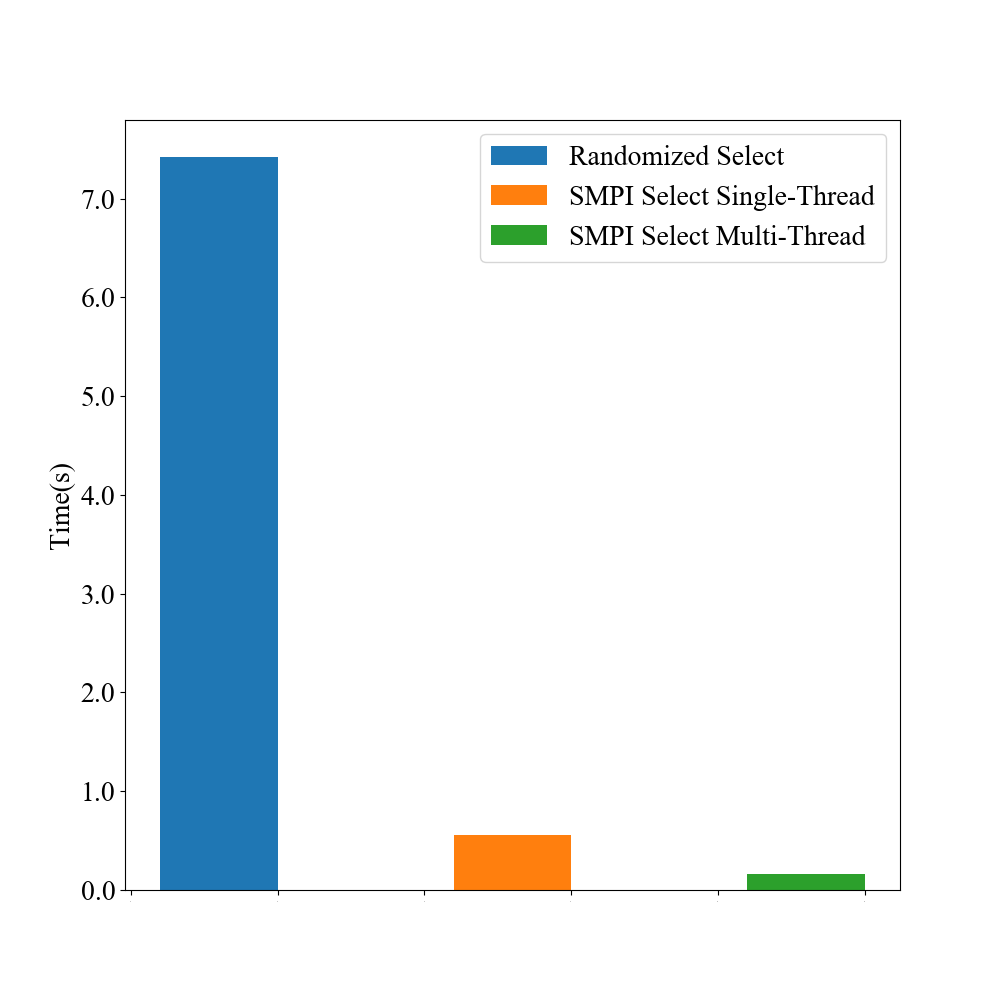
\includegraphics[width = 15cm]{select-time.png}
    \caption{第k大梯度选择过程时间}
    \label{fig:select}
  \end{figure}

可以看出,本文的优化大幅度缩短了选择第k大梯度所用时间,可以在单线程和多线程下分别将性能提升13.3倍和46.0倍。这些加速主要来源于输入随机选择算法中的元素数目的减少。由于随机选择算法本身非常难以使用并行计算加速,所以通过采样来减少输入随机选择算法中的元素数目的同时,也为并行加速采样过程提供了机会。

在接下来的所有测试中,Allreduce算法中的第k大梯度的选择过程均使用优化后的算法进行测试。

之后,我们测试了Open MPI与SMPI分别执行Allreduce算法所用时间,如图\ref{fig:ompi-vs-smpi}所示。测试所用的缓冲区大小为1 MB $\sim$ 2 GB,并将TCP的Open MPI 的Allreduce时间作为1,将使用RDMA的Open MPI、使用TCP的单线程SMPI以及使用TCP的多线程SMPI 的Allreduce时间分别与其进行对比,Y轴数值越小,所用时间越少。

\begin{figure}[ht] % use float package if you want it here
    \centering
    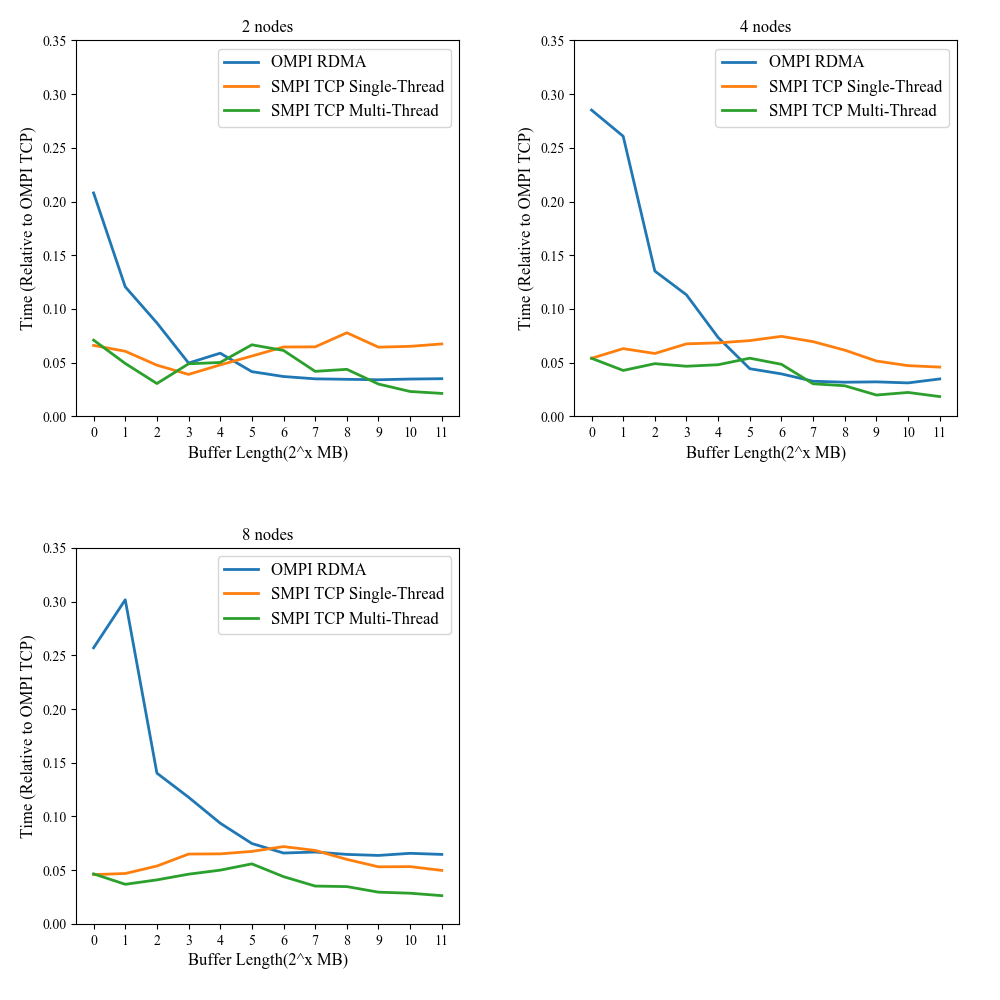
\includegraphics[width = 15cm]{ompi-vs-smpi.png}
    \caption{Open MPI 与 SMPI执行 Allreduce 算法时间对比}
    \label{fig:ompi-vs-smpi}
  \end{figure}

在缓冲区较大时,多线程版本的SMPI与使用RDMA的Open MPI性能相当,都可以比使用TCP的Open MPI快20 $\sim$ 30倍,这说明优化后的稀疏矩阵Allreduce算法即使在网络带宽较低的情况下依然可以媲美使用了高带宽网络的传统Allreduce算法;而单线程版本的SMPI则相对稍慢一些,这是因为随着缓冲区长度增加,稀疏矩阵的压缩、解压缩以及第k大梯度的选择过程所用时间明显增长,通过多线程并行计算可以得到明显的加速效果。

在节点数为8时,多线程版本的SMPI性能全面超越使用RDMA的Open MPI,它的性能是使用TCP的Open MPI的性能的38.0倍,是使用RDMA的Open MPI的性能的2.5倍。相对于Open MPI而言,SMPI的相对时间随着节点数的增多而变得更少,这足以说明本文的算法具有良好的可扩展性。

我们也可以看到,在节点数相同时,SMPI的相对时间随着缓冲区长度的增加而明显减少,这说明本文设计的算法更适合参数较多的神经网络模型。由于一般只有参数较多的模型才需要进行分布式训练,所以本文的算法效果与设计初衷是相符合的。

接下来,我们对SMPI Allreduce算法进行了详细分析。如图\ref{fig:breakdown-smpi-singlethread},这是单线程的SMPI Allreduce算法中各部分的占用时间;如图\ref{fig:breakdown-smpi-multithread},这是多线程的SMPI Allreduce算法中各部分的占用时间。测试所用的缓冲区大小为2 GB。

\begin{figure}[ht] % use float package if you want it here
    \centering
    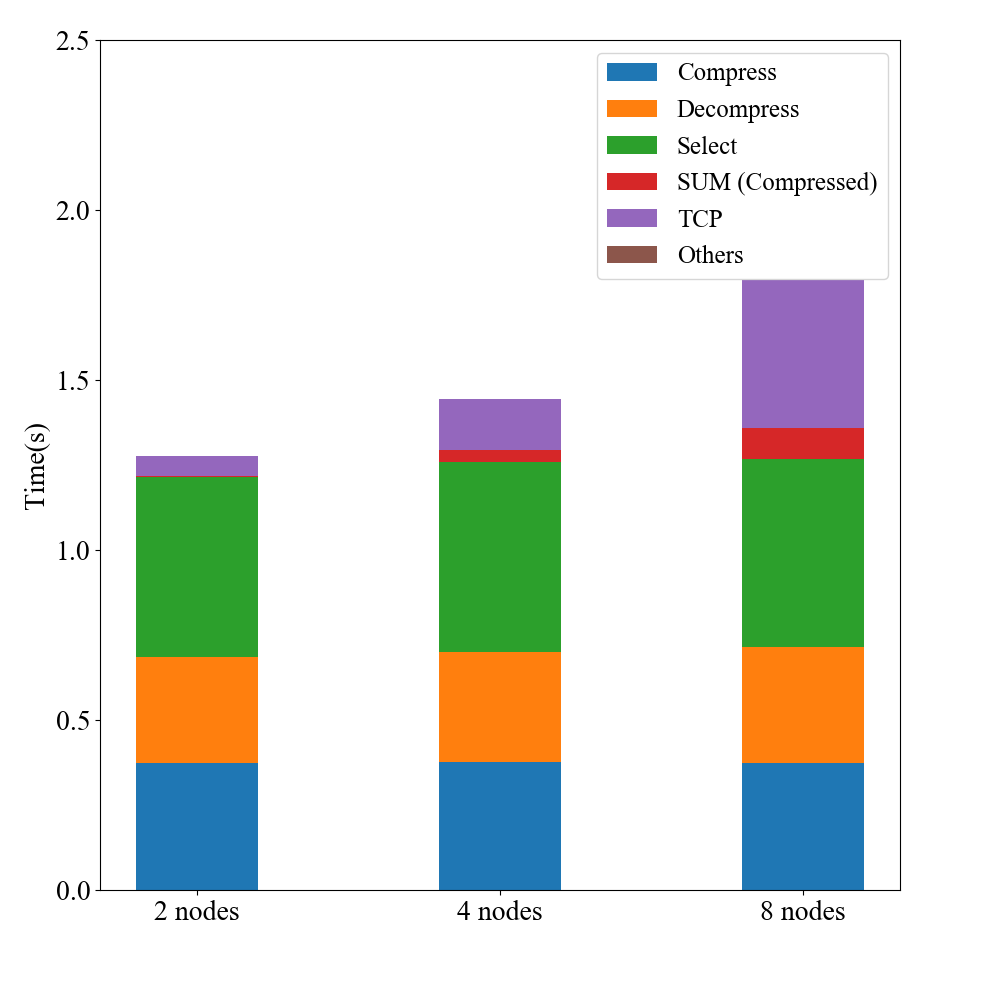
\includegraphics[width = 15cm]{breakdown-smpi-singlethread.png}
    \caption{单线程SMPI Allreduce详细分析}
    \label{fig:breakdown-smpi-singlethread}
  \end{figure}

  \begin{figure}[ht] % use float package if you want it here
    \centering
    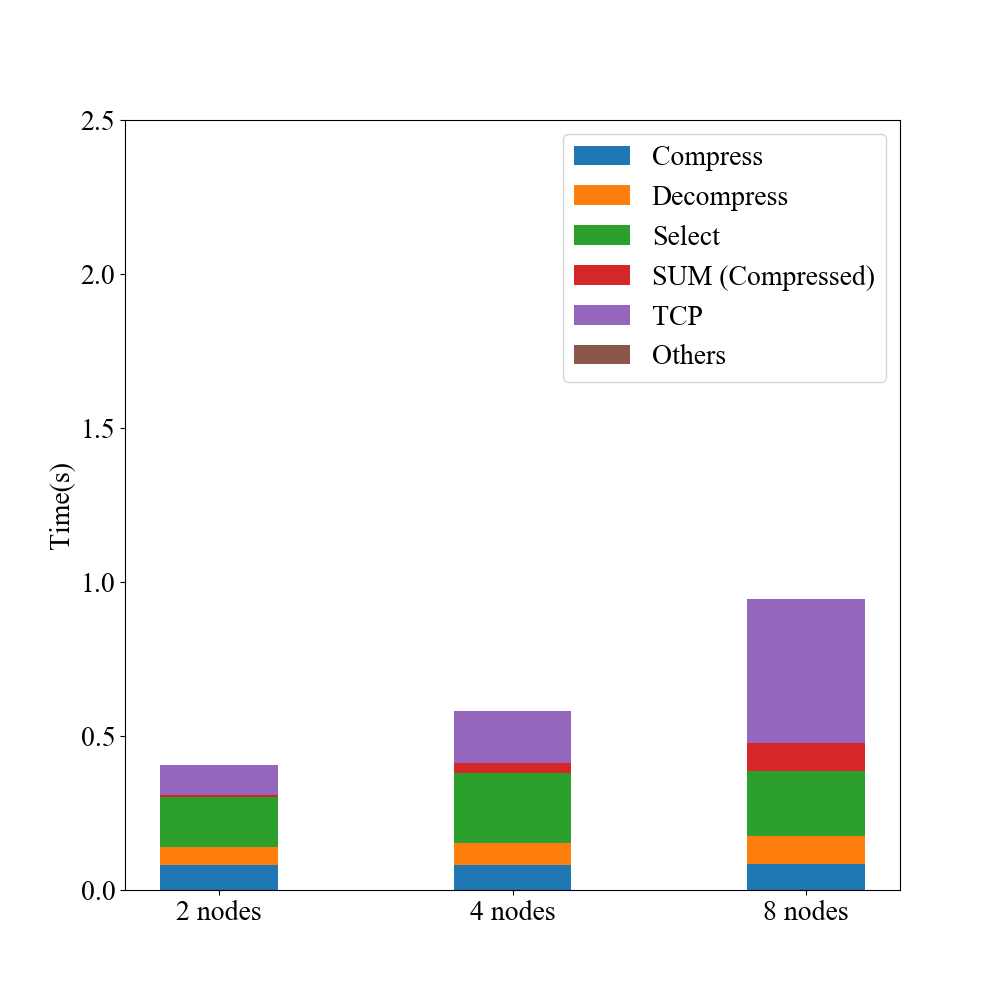
\includegraphics[width = 15cm]{breakdown-smpi-multithread.png}
    \caption{多线程SMPI Allreduce详细分析}
    \label{fig:breakdown-smpi-multithread}
  \end{figure}

可以看到,在只使用单线程的时候,第k大梯度的选择与稀疏矩阵的压缩、解压缩等计算过程占据Allreduce算法的大部分时间,尤其是第k大梯度的选择,在只有两个节点的时候占据50\%左右的时间。同时,除了稀疏矩阵加法之外的这些计算操作,只在Allreduce算法的开始或结束时执行一次,并不参与每轮的通信过程,与通信轮数和节点个数无关,它们的计算时间并不会随着节点数变多而增加,这也是本文的算法能够具有良好的扩展性的原因之一。

在使用多线程加速之后,计算相关的操作所占时间明显减少,压缩、解压缩和选择时间分别降为单线程时的22.9\%、26.5\%和38.0\%。在这三者中,依然是第k大梯度的选择所用时间最多,同时,它的加速效果也相对较差。这是因为选择过程中需要调用随机选择算法,而我们难以对该算法使用多线程加速。

最后,我们将SMPI的普通模式与智能网卡模式进行对比,如图\ref{fig:smpi-smartnic}所示。

\begin{figure}[ht] % use float package if you want it here
    \centering
    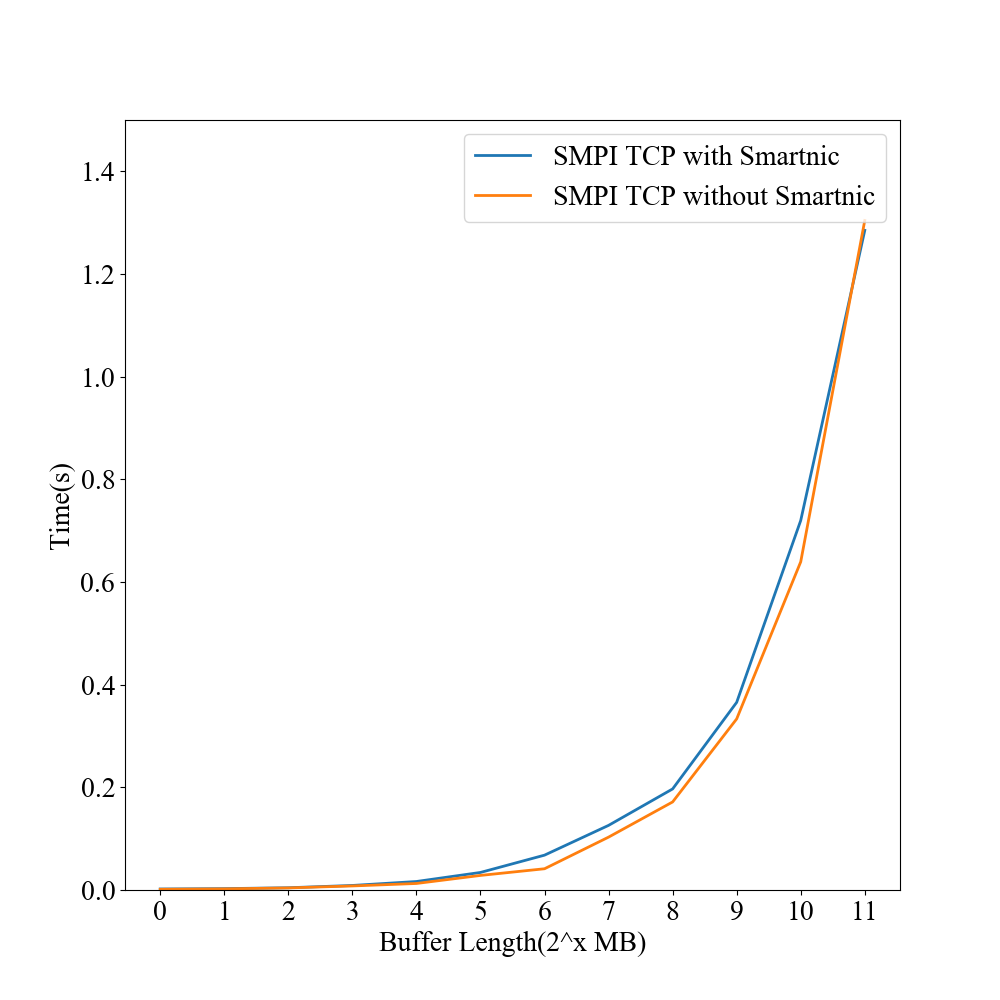
\includegraphics[width = 15cm]{smpi-smartnic.png}
    \caption{SMPI 普通模式与智能网卡模式对比}
    \label{fig:smpi-smartnic}
  \end{figure}

由于硬件限制,目前只使用了两个节点进行测试。通过结果可以看出,普通模式与智能网卡模式的性能基本持平,但普通模式的性能略微好一些,这是因为目前只使用了两个节点,Allreduce算法只需要通信一轮,即使使用了智能网卡也无法得到降低延迟的益处;同时,由于在通信开始前,需要将稀疏矩阵显式地由主机端发送至网卡,并在通信结束后由网卡发回主机,多了一些系统调用的额外开销,导致性能略微降低。

由于只使用了两个节点,无法验证使用智能网卡可以降低延迟的特性,希望以后的工作可以将此实验完善。

\subsection{Pytorch 分布式训练性能测试}
我们将自己的算法移植至Pytorch的后端---Gloo---进行神经网络的分布式训练,并与Pytorch自带的分布式训练进行对比。图\ref{fig:breakdown-pytorch}为分布式训练一个Batch的所用时间,其中相邻两个柱状图的左侧为原Pytorch的分布式训练所用时间,右侧为使用本文的算法优化后的Pytorch的分布式训练时间。蓝色部分表示Allreduce算法占用时间,橙色部分表示其余所有时间,包括正向传播算法、反向传播算法以及模型参数的更新等。

\begin{figure}[ht] % use float package if you want it here
    \centering
    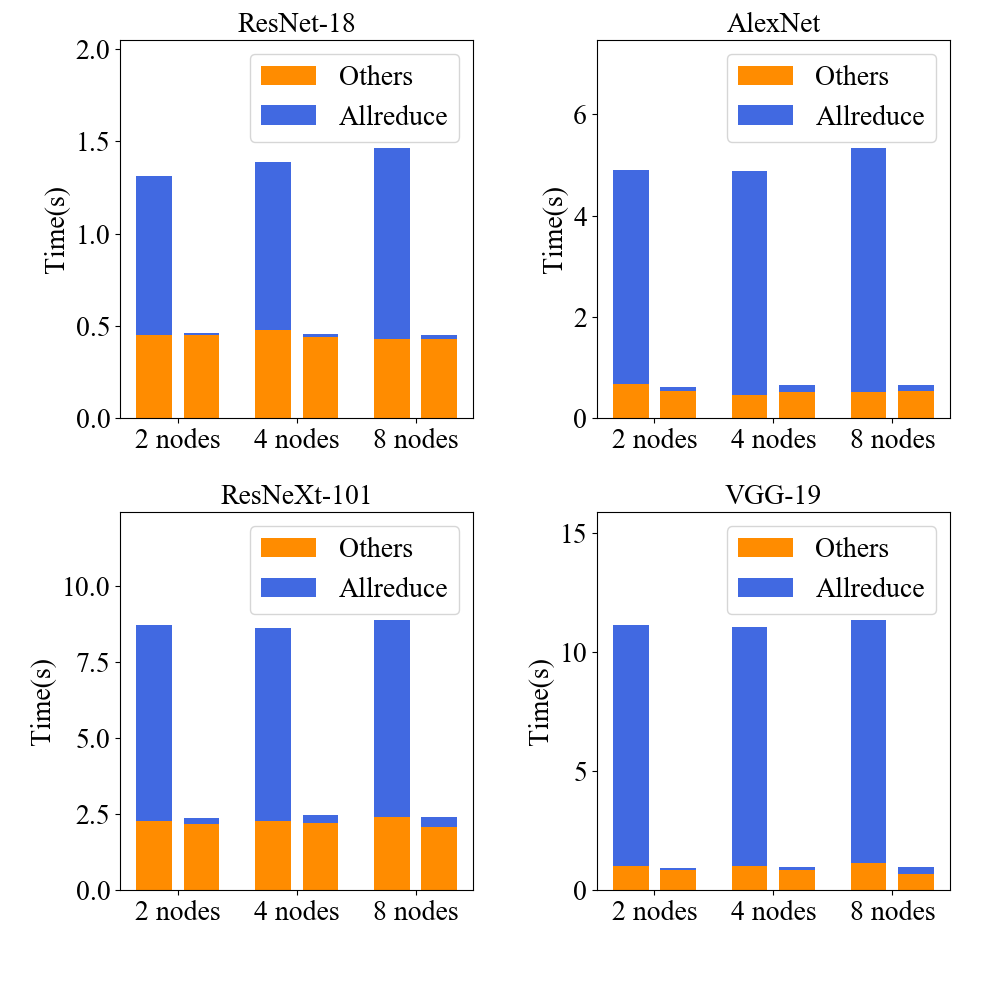
\includegraphics[width = 15cm]{breakdown-pytorch.png}
    \caption{分布式训练时间对比}
    \label{fig:breakdown-pytorch}
  \end{figure}

可以看出,优化后的分布式训练中Allreduce所占时间非常少,且随着节点数的增多,Allreduce所占时间变化不大,这说明本文的算法在真实的神经网络分布式训练中依然有非常好的可扩展性。

由于神经网络中不同层的计算量与参数的比值不一致,比如卷积层的参数很少但计算量很大,所以不同网络的计算--通信比是不一样的。比如,图\ref{fig:breakdown-pytorch}中AlexNet网络的计算--通信比大约只有9.4\%,而ResNet-18的计算--通信比则有29.3\%。神经网络的计算--通信比越小,也就意味着通信时间所占比例越大,在使用本文的算法进行优化后,得到的性能提升也就越高。经过测试,ResNet-18、AlexNet、ResNeXt-101和VGG-19的分布式训练性能分别提高了3.3倍、8.3倍、3.7倍和8.6倍。

